% status: 100
% chapter: Security

\title{Service for Managing the Public Key}

\author{Uma M Kugan}
\affiliation{%
  \institution{Indiana University}
  \streetaddress{107 S. Indiana Avenue}
  \city{Bloomington}
  \state{Indiana}
  \postcode{43017-6221}
}
\email{umakugan@iu.edu}
% The default list of authors is too long for headers}

\renewcommand{\shortauthors}{Uma Kugan}
\begin{abstract}
SSH keys are used to control access to any system using public and private
key pair. The user creates the private keys and store it securely on his 
machine and shares the public key. Usually IT admins distributes and
manage SSH keys which creates more hassle for the admins to manage.
In this paper, we are going to create a rest service to manage their
public key.

\end{abstract}

\keywords{hid-sp18-513, Security, Key Management}


\maketitle

\section{Introduction}
SSH is a way for anyone to connect to any servers in a more secured way. 
Any information that is exchanged between host computer to the server is
encrypted which prevents someone from snooping the data. There are two
ways by which user can authenticate to connect to the servers: one by
providing user name and password combination or by using SSH keys.
SSH keys are used in most organizations. The problem with SSH keys is keeping 
track of whose SSH key has been placed on which machines and making sure that 
the keys get changed every couple of days/weeks so that it is hard for anyone 
to guess what the key Is and try to attack the server by forging your 
identity. One of the main issues is that IT admins have to spend a lot of 
time visiting each server, changing out the private keys then go back to each
user and have them make changes on their laptop
~\cite{hid-sp18-513-ylonen2013user}. 
The rest api provides the easier solution to exchange keys between the servers
and in this project we have created few api to transfer keys between servers
and also to properly manage them.

\subsection{What is SSH?}
The SSH protocol encrypts to secure the connection between a
client and a server. All user authentication including commands,
results and file transfers are encrypted to protect against attacks
in the network.

\begin{figure}[!ht]
        \centering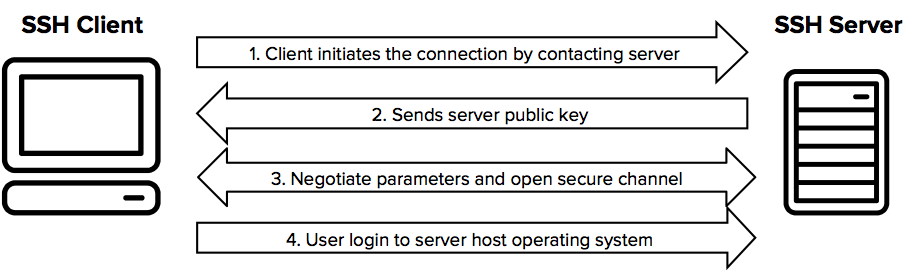
\includegraphics[width=\columnwidth]
        {image/ssh-protocal.png}
        \caption{SSH Protocol~\cite{hid-sp18-513-sshkeyinc}}\label{fig:figure1}
\end{figure}

\section{How SSH Works}
SSH uses a client-server model of computing, allowing users to establish
secure communications between two hosts, whether UNIX, Windows
or virtually anything else. SSH is also increasingly important as the use
of cloud computing grows, helping organizations limit exposure while
connecting to a cloud-based virtual machine over the Internet by providing
a local gateway-style system via an SSH endpoint.
The server enables incoming SSH connections to a host and handles user
authentication, authorization and related tasks. The client connects to an
SSH server and makes requests after authenticating to the server. 
An SSH session is the ongoing connection between a client and a server begins
after the client successfully authenticates to a server and ends when the
connection terminates. Once the system authenticates a user, one or more
channels may be opened within the connection, with each channel acting
as an individual data link and separate pathway for information
~\cite{hid-sp18-513-sans}.


\section{Role of Secure Shell}
The Secure Shell (SSH) protocol, developed in the mid-1990s, and it  
used everywhere both in traditional and virtual environments to 
authenticate Unix users and their applications to remote, 
internal systems and encrypt the resulting session traffic. 
In order to authenticate, an user or an application must share
its private SSH key file to a target system that possesses its 
corresponding public SSH key file. 
Once the key pair is validated, the user or application is granted 
access to the protected account. In effect, this means that any user
or application with access to a private key may access any target 
system such as Unix and Linux systems, virtual machines, network 
devices, or file transfer solutions that contains the corresponding
public key.
In a one-to-many environment, in which one private SSH key is used 
to attain privileged access to many target systems, organizations 
can no longer afford to ignore these privileged private keys. 
To protect the heart of the enterprise,organizations must 
proactively secure and manage all of their privileged account 
credentials, including both passwords and SSH keys, to achieve
consistent, comprehensive protection against advanced 
attacks~\cite{hid-sp18-513-cyberark}

\section{SSH Key}
SSH keys are basically files that are generated by the OpenSSH program on
any computer. An SSH Key consists of two parts. A public key and a private 
key. An SSH key is an access credential in the SSH protocol in which
keys are primarily used for login to one server from other server 
without entering the passwors and it is also used in automated processes
and used by system administrators for implementing single sign-on.

\subsection{Private and Public Key}

The private key file is kept hidden usually in the home directory 
which can be accessed when connecting to a server. The public key is placed 
on the server that we are trying to get access to. Now, when we try to 
connect to the server, computer presents information to the server via the 
SSH key that proves to the server its really you trying to get access. 
Without the public SSH key on the server and private key on the computer
nobody can access your account using SSH~\cite{hid-sp18-513-sshkeyinc}.


\subsection{Authorized Key}
An authorized key in SSH is a public key used for granting login access
to users and this authentication mechanism is defined as public key 
authentication. Authorized keys is the file that contains public 
key of the other server from which passwordless sign on can be 
initiated and it is configured separately for each user. It is 
usually present in .ssh under home directory. 
Key location and name are editable in SSH server configuration 
files. To properly secure and manage, it is usually named same as 
root owned location~\cite{hid-sp18-513-sshkeyinc}.
A key pair can be created using the ssh-keygen in openssh and then
the public key is copied to server using ssh-copy-id tool.

\section{What is SSH-Keygen}
Ssh-keygen is a tool for creating new authentication key pairs 
for SSH. SSH supports several public key algorithms for creating
authentication keys. 

\subsection{RSA}
It is an old algorithm based on the difficulty of factoring large 
numbers. It is quite possible the RSA algorithm will become 
practically breakable in the foreseeable future and hence it is 
advisable to choose some other algorithm. All SSH clients support
this algorithm~\cite{hid-sp18-513-sshkeyinc}.

\subsection{DSA}
It is an old US government Digital Signature Algorithm which is
based on the difficulty of computing discrete logarithms. 
DSA in its original form is no longer recommended
~\cite{hid-sp18-513-sshkeyinc}.

\subsection{ecdsa}
A new Digital Signature Algorithm standardized by the US government,
using elliptic curves. This is probably a good algorithm for current
applications. Most SSH clients now support this algorithm
~\cite{hid-sp18-513-sshkeyinc}.

\subsection{ed25519}
This is a new algorithm added in OpenSSH. Support for it in clients
is not yet universal~\cite{hid-sp18-513-sshkeyinc}. 

\section{SSH-COPY-ID}
ssh-copy-id installs an SSH key on a server as an authorized key. 
Main use of SSH Copy Id is to provision access without prompting
the user for the password. The ssh copy id command edits the 
authorized keys file on the server. It creates the .ssh directory 
if it does not exist and it also creates the authorized keys file
if it does not exist and then ssh key is copied to server.

\section{SSH Client Configuration Files}
The ssh program on a host receives its configuration from either
the command line or from configuration files:
\begin{itemize}
\item ~/.ssh/config
\item /etc/ssh/ssh\_config
\end{itemize}

ssh command gets the configuration data from the below three 
mentioned sources in the order they are stated:

\begin{itemize}
\item command line options
\item user-specific configuration file (~/.ssh/config)
\item system-wide configuration file (/etc/ssh/ssh\_config)
\end{itemize}
~\cite{hid-sp18-513-sshkeyinc}. 

\section{SSH-COPY-ID}
ssh-copy-id installs an SSH key on a server as an authorized key. 
Main use of SSH Copy Id is to provision access without prompting
the user for the password. The ssh copy id command edits the 
authorized keys file on the server. It creates the .ssh directory 
if it does not exist and it also creates the authorized keys file
if it does not exist and then ssh key is copied to server.

\section{SSH Agents}
If private key is encrypted with a passphrase, then passphrase
must be entered every time to connect to an SSH server using
public-key authentication. Whenever the ssh or scp command is
executed, the server will need the passphrase to authenticate
and to decrypt the private key before it lets into the remote
server.

An SSH agent is a program used to decrypt the private
keys and provide access to SSH client programs. User need to
provide passphrase once, when adding your private key 
to the agent's cache. This is used when frequent SSH connections
are made. An agent is typically configured to run automatically 
upon login and persist for the duration of your login session. 
SSH-Agent is the default agent included with OpenSSH
~\cite{hid-sp18-513-sshkeyinc}.

\section{SSH Keys: The Hidden Credentials} 
SSH keys are always the major concern to security teams because 
these credentials can be easily created, and are then difficult to
track, manage or control. In any environment without any proper
controls in place, any user with access to any machine can generate
an SSH key pair that will forever grant that user direct access to
the system. And, because there is no built-in oversight to SSH keys,
no one may ever know. Further, because SSH is commonly used in 
automated application to application authentication,
SSH key pairs can be generated, distributed and never thought of again, 
leaving applications and application servers vulnerable to attacks 
using unmanaged, outdated SSH keys~\cite{hid-sp18-513-cyberark}. 
In the enterprise environment with hundreds of IT users and 
thousands of systems managing the SSH challenge becomes exponential. 
A large enterprise may have thousands or even millions of valid 
SSH key pairs, many of which may no longer be needed by authorized 
users or applications. As a result, attackers can exploit this 
vulnerability and gain privileged access to critical systems. 
Without central management or knowledge of who 
is accessing what, organizations cannot see where their risks and
vulnerabilities lie much less take action to address them
~\cite{hid-sp18-513-cyberark}. 

\section{SSH Keys Vulnerabilities}
Vulnerabilities with SSH range from weaknesses in the protocol
itself to configuration, implementation and management 
complexities that can lead to dangerous mistakes.
Poor SSH key management practices can result in compromise 
of administrative privileges, expanded breadth of attack surfaces
and other issues that could easily be avoided by proper training
and more effective processes backed by automation and tools
~\cite{hid-sp18-513-sans}.

\subsection{Configuration Issue}
Application developers must learn how to keep both configuration
and private key files secure. With these files, a malicious 
individual can easily impersonate an authorized
user (or host) and easily connect to a remote host and application.
Before deploying any new devices in a networked environment,
it is always the best practice to change default passwords
for all applications, operating systems, routers, firewalls
and all other systems~\cite{hid-sp18-513-sans}.

\subsection{Gaining Access with SSH Key}
Lack of defined governance for SSH key-based trust 
relationships can allow an attacker who compromises one 
system to quickly pivot from one system to another and extend
a breach into other parts of an organization. Enough keys may be 
stolen, leaked or misused without having terminated their trust
relationships to pose a serious, ongoing threat to an organization.
Attackers once get access to these keys, they will generates a new 
key pair and adds the new authorized key to authorized keys file
which is not usually monitored or audited.
The December 2014 Sony hack included the leak of SSH keys as well
as password lists, which led to the compromise of related services and
accounts; mishandled SSH keys may have even facilitated the initial 
compromise~\cite{hid-sp18-513-sans}.

\section{How to Manage SSH Risks?}
To reduce the threat and comply with regulatory requirements, 
organizations should take a proactive, end-to-end approach to SSH key
security and management. Such an approach should include proactive
controls to secure, manage and monitor the creation, storage and use
of all privileged SSH keys. By employing a layered approach that includes
the critical security measures outlined below, organizations can build
out a proactive SSH key management program that reduces risks and helps 
meet regulatory requirements.

\subsection{Secure Key storage}
To reduce the risk of stolen SSH keys, organizations should store 
private user and application keys in a highly-secure
centralized repository that supports strong access controls.
In an unmanaged state, SSH keys are stored as system files and can 
easily be moved or copied. As a result, critical systems are only
as secure as the machines or devices on which the private keys are
stored. To mitigate this risk, organizations should consider removing
SSH keys from vulnerable endpoints and systems and instead storing 
them in a highly secure, highly available central repository that 
supports access controls such as automated workflows for 
elevated-privilege requests and strong authentication to quickly 
verify user and application identities. With a secure centralized 
model, organizations can remove critical credentials from individual
machines, protect all credentials equally and centrally track all usage
of SSH keys by users and applications~\cite{hid-sp18-513-gutmann}.

\subsection{Proactive key rotation}

Similar to static passwords, static SSH keys pose an on-going risk
to organizations. Compromised private SSH keys can provide unauthorized
users with permanent backdoor access into critical systems. 
To mitigate this risk, organizations should rotate all SSH key 
pairs at regular intervals, just as they rotate privileged passwords
today. In unmanaged environments, with keys dispersed across devices,
the prospect of frequently rotating thousands of keys can be daunting.
However, once all user and application SSH keys are consolidated under
one central management system, key pairs can be automatically rotated
and public keys can be automatically distributed to target systems. 
With central management and automated key rotation, organizations can
better secure SSH keys and the target systems they protect, 
implement best practices and comply with regulations without burdening
the IT team\cite{hid-sp18-513-gutmann}.

\subsection{Privileged Session monitoring}

Proactive protection of privileged credentials is a critical element
in privileged account security, but proactive controls must be 
complemented with equally strong detection and response capabilities.
To minimize any potential damage caused by advanced external and
inside attackers, organizations should proactively monitor all
privileged sessions, including those that occur via SSH. When abnormal
activity is detected, security teams should have the ability to
remotely terminate the suspicious session to disrupt the potential attack.
Similarly, organizations must also record all privileged session activity.
When an incident is detected, response teams require immediate access to
session recordings and detailed audit logs to determine exactly what
happened and what steps must be taken to re-mediate the incident.
Access to these privileged session recordings and audit logs can also be
granted to auditors to help prove compliance with regulations
~\cite{hid-sp18-513-gutmann}.

\section{Measures to be taken for Securing SSH Keys}

Both internal and external auditors must add Secure Shell key 
scanning and management to their checks. Proper controls and tools
must be put in place for managing Secure Shell keys. The real issue
is authorized keys, as they are the ones that grant access. No
matter how much you try to protect private keys, it is of no help 
until the millions of existing authorized keys have been sorted out.
Regulators must establish firm deadlines for enterprises and execute 
the revoking of all access when no longer needed. However, 
implementation and audit guidelines should be clarified
to ensure Secure Shell keys are taken into account. Boards, 
audit committees, Security and Governance and risk management 
officers must ensure Secure Shell key-based access is
properly accounted for in their organizations to avoid civil 
and criminal liability~\cite{hid-sp18-513-network}.

\subsection{Use Passphrase}

It is always recommended that keys used for single sign-on should 
have a passphrase to prevent use of the key if it is stolen or 
compromised. It is the best practice to use keys without
passphrase for fully automated jobs such as backups.

The ssh-agent and ssh-add programs can be used to avoid having to 
enter the passphrase every time the key is used.

\subsection{Command Restrictions}

A command restriction is a command=``<permitted command>'' option
added to the beginning of the line in the target server authorized
keys file.  The copy-id tool does not default any restrictions but it
is highly recommended when the key is used for automating operation.

\section{NIST ISSUES GUIDANCE ON SSH KEY MANAGEMENT}
US National Instute of Standards and Technology (NIST) as issued guidance on
SSH key management as NIST IR 7966. 

\subsection{REGULATORY COMPLIANCE REQUIRES SSH KEY MANAGEMENT}
Typical requirements for compliance include:
\begin{itemize}
	\item Managing Identities and Credentials - SSH keys 
	are access credentials
	\item Provisioning and Termination Process for Access 
    - including access based on SSH keys
	\item Segregation of Duties - elimination of 
	key-based access from test and development systems into
	production
    \item Disaster Recovery - limiting attack spread
    from primary systems to disaster recovery sites and
    backup systems
    \item Privileged Access Controls - SSH keys are often used to 
    bypass jump servers
    \item Boundary definition and documentation of connections for 
    systems that contains sensitive data such as payment systems,
    financial data environments, patient data 
    environments, or between government information systems
    \item Incident Response and Recovery
\end{itemize}
~\cite{hid-sp18-513-sshkey}.

\section{Python - API}
Python is a high-level object-oriented programming language which 
is most popular and widely used due to its minimal setup and high
availability of large collection of free libraries. The project 
uses Python 2.7 that is available in the native version of 
Ubuntu 16.07.

\subsection{Flask - Rest Service}
Flask is a micro framework developed for web development. The 
framework is widely popular because its light weight and has 
minimal dependencies. Flask was originally written in Python. 
Some of the key features of Flask are integrated rest service,
secure cookies and unit testing support. Flask-RESTful is an
extension of Flask that supports quick and easy API
deployments with minimal setup. 

\section{Deployment}
The Project uses few API to effectively manage the keys and their
user authorization in Sqlite Database.
Three tables have been created to maintain access request and also
the list of users in each server, their groups and their access level.

\subsection{Setup}
\paragraph{Git repository}
Setup the git repository:
\begin{verbatim}
export HID=hid-sp18-513 
mkdir -p ~/github/cloudmesh-community
cd ~/github/cloudmesh-community 
git clone
https://github.com/cloudmesh-community/$HID.git
/project-code
\end{verbatim}

Technology: Python, Flask API, Sqlite3

Install \textbf{Python 2.7.13} via PIP

Install \textbf{pip install flask-restful} 

Database: sshkeymgmt.db 

Tables: usergrp, user access, user\_req\_access 

API: 
    /\verb|request_access|

    /\verb|validate_and_action|

    /\verb|create_ssh_key|

    /\verb|copy_ssh_key|

User will call the API request access to request for sharing 
the key from one server to other server with host name and 
user id of the source and target and also the location of 
public key in source host.

API validate and action will validate if the user have a 
login in the target server. If not the request will be declined
and the status will be updated on the table.

Once the request is approved, the third API will actually copy
the keys to target server. Before it copies, API will validate
if the user calling the API have access to target server or
whether he is any group and or has admin access. 

If key is not present, \verb|create_ssh_key| api can be used to
create the ssh key.

Getstatus api is used to get status of the request at any point,
user need to pass the status: APPROVED, DENIED, COMPLETED, FAILED.

\section{SSH Key Management Products}

There are several SSH Key Management Products that are readily available
in the market. These products will help to generate, manage, store and
rotates the key periodically. SSH.com's Universal Key Manager is the
industry's leading product which provides risk assessments, process driven,
full control and all in one view. There are other products such as 
FOXPASS which can integrate with LDAP server.

\section{Limitations}

In this project, we have define a very basic api to manage the ssh keys.
This project can be further enhanced and extended to include active directory 
or LDAP integrations.


\section{Conclusion}

SSH is an widely used important protocol that provides encrypted, 
authenticated communications in a variety of configurations. Public key
authentication is very vital to any organization, as it automates 
access and can easily provide ease of login to accounts with elevated 
privileges. However, SSH is also especially vulnerable to complexities
that involve configuration, implementation and management. In order to
reduce risk, proactive monitoring and implementation of best practices 
both during implementation and afterward is needed. 

In a big organizations, there may be huge volumes of keys in use and
remediation of an environment where SSH keys and trust relationships 
have never been fully managed is complex, labor-intensive and 
time-consuming. But there are frameworks available in the industry which 
can be used or the project has few basic API to manage the key in smaller 
environment which can be further enhanced to larger scale.


\begin{acks}
The author would like to thank Dr.~Gregor~von~Laszewski for his support and 
suggestions in writing this report and succesfully completing the project.
\end{acks}

\bibliographystyle{ACM-Reference-Format}
\bibliography{report}







